\documentclass{beamer}

\usepackage{amsfonts}
\usepackage{amsmath}
\usepackage{longtable}
\usepackage{csquotes}
\usepackage{standalone}

\usepackage{graphicx}
\graphicspath{{../pictures/}}

\usepackage{tikz}
\usetikzlibrary{shapes, calc, arrows, decorations.markings,
  decorations.pathmorphing, decorations, patterns, chains, snakes,
  backgrounds, positioning, fit, petri}
\newcommand{\inputpicture}[1]{\input{../drawings/#1}}

\usepackage{listings}
\lstset{language=C, basicstyle=\ttfamily, breaklines=true, keepspaces=true,
  keywordstyle=\color{blue}}

\usepackage{bytefield}

\usefonttheme{professionalfonts}
\usefonttheme{serif}
\usepackage{fontspec}
\setromanfont{CMU Serif}
\setsansfont{CMU Sans Serif}
\setmonofont{CMU Typewriter Text}

\usepackage{hyperref}
\hypersetup{colorlinks=true, linkcolor=black, filecolor=black, citecolor=black,
  urlcolor=blue , pdfauthor=Evgenii Iuliugin <yulyugin@gmail.com>,
  pdftitle=Fundamentals of Full-Platform Simulation}

\usepackage{underscore}
\usepackage{amsthm}

\subtitle{Fundamentals of Full-Platform Simulation}
\subject{Lecture}
\date{\today}

\author[Evgenii Iuliugin]{
  Evgenii Iuliugin \small{\href{mailto:yulyugin@gmail.com}{yulyugin@gmail.com}}}
\typeout{Copyright 2021 Evgenii Iuliugin}

\usetheme{Berlin}
\setbeamertemplate{navigation symbols}{}

\newcommand{\finalslide}{
    {\huge{Thank you!}\par}

    \vfill
    Slides and material are available at
    \url{https://github.com/yulyugin/sim-lectures}
    \vfill

    \tiny{\textit{Note}: All trademarks are the property of their respective
        owners.
        The presented point of view reflects the personal opinion of the author.

        %All the materials are licensed under the Creative Commons
        %Attribution-NonCommercial-ShareAlike 4.0 Worldwide. To view a copy of
        %this license, visit
        %\url{http://creativecommons.org/licenses/by-nc-sa/4.0/}.
    }
}

\title{Paravirtualization --- Connecting Real Word With Simulation}

\begin{document}

\startslides

\begin{frame}{На прошлых лекциях}

Изоляция + эквивалентность $\neq$ эффективность

\begin{itemize}
\item Мы стремились к наиболее точной симуляции. Программы в гостевом окружении не должны догадываться, что они исполняются не на реальной аппаратуре
\item Они не должны знать о мониторе ВМ
\item Цена этому — скорость работы

\end{itemize}

\end{frame}

\begin{frame}{Вопросы по предыдущей лекции}

\begin{itemize}
\item Какие три признака эффективного монитора ВМ сформулированы Г. и П.?
\item Что такое безвредные (innocuous) инструкции?
\item Что такое и как используется SLAT (second level address translation)?

% \item Что такое «каузальность»?\pause
% \item Дайте определение понятию GVT \pause
% \item Может ли параллельная модель быть детерминистичной? %\pause

\end{itemize}

\end{frame}

\begin{frame}{На этой лекции}

\begin{itemize}
% \item Иногда удобно/выгодно взаимодействовать между уровнями 
\item Взаимодействие виртуальности с реальностью
\item Паравиртуализация 
% \item Гостевые расширения
% \item Сетевые сервис-точки
\end{itemize}

\end{frame}

\section{Изоляция против производительности}

\begin{frame}{Зачем}

\begin{itemize}
\item Иметь возможность передавать данные в/из симулируемой системы
\item Более эффективно \emph{совместно} работать над управлением ресурсами машины:
память, время, устройства
\item Иметь возможность передавать аппаратные ресурсы частично или полностью в VM
\end{itemize}

\end{frame}


\begin{frame}{Связи между гостем и хозяином}

\begin{tikzpicture}[>=latex, font=\small, node distance=0.3cm, inner sep=0pt]
    
    \node (tower) {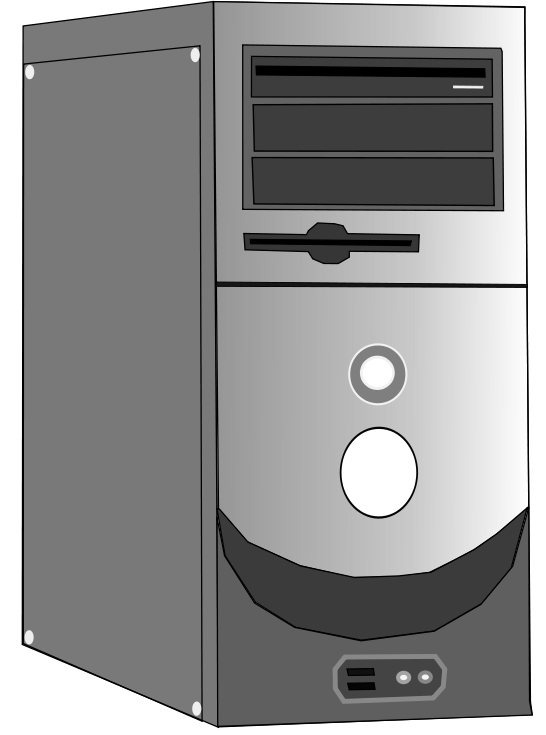
\includegraphics[height=1.5cm]{./tower.png}};
    \node[above=of tower] (monitor1) {
\includegraphics[height=1.2cm]{./monitor1.png}};
    \node[right =0.2cm of monitor1] (kb1) {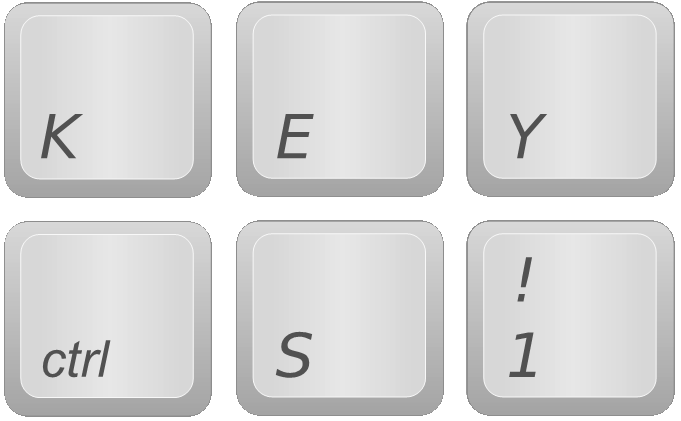
\includegraphics[height=.8cm]{./kb1.png}};
    
    % Inner border
    \node[draw, inner sep=0.2cm, fit=(tower) (monitor1) (kb1)] (virt) {};
    
    \node[right =2.cm of tower] (folder) {
\includegraphics[height=1.cm]{./folder.png}};
    \node[right =0.2cm of folder] (hdd) {\includegraphics[height=1.cm]{./device3.png}};
    
    \node[right=0.7cm of hdd] (stub) {};
    
    % The outer border
    \node[draw, inner sep=0.35cm, fit= (virt) (tower) (monitor1) (kb1)  (hdd) (stub)]  (real) {};
    
    \node[right =0.2cm of hdd] (nic) {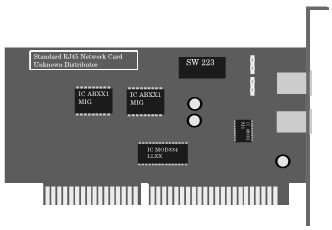
\includegraphics[height=1.cm]{./nic.png}};
    \node[right =of kb1, yshift=1cm] (kb2) {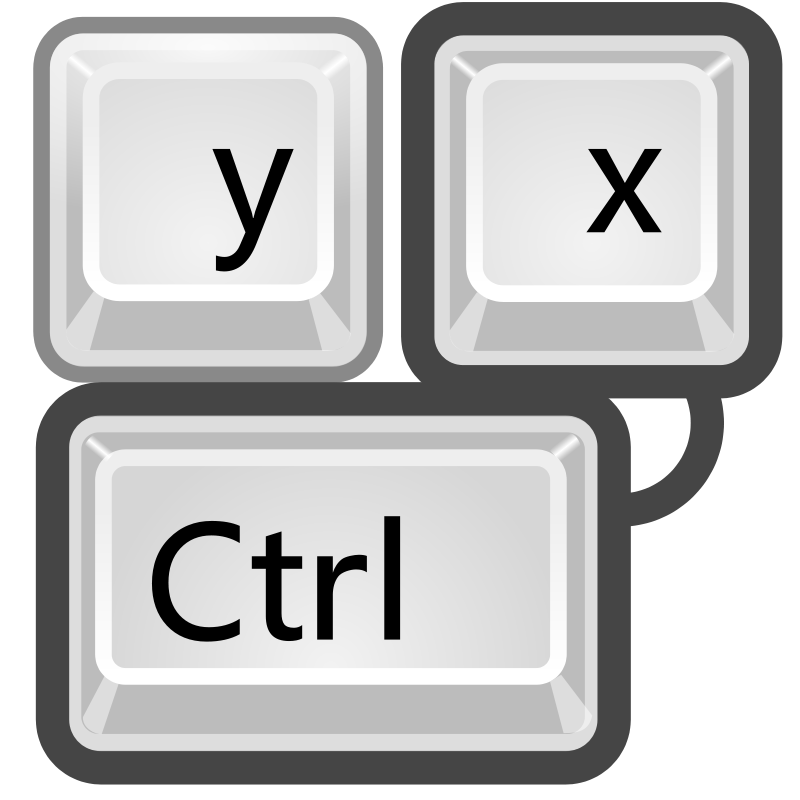
\includegraphics[height=1.5cm]{./kb2.png}};
    \node[right =of kb2] (monitor2) {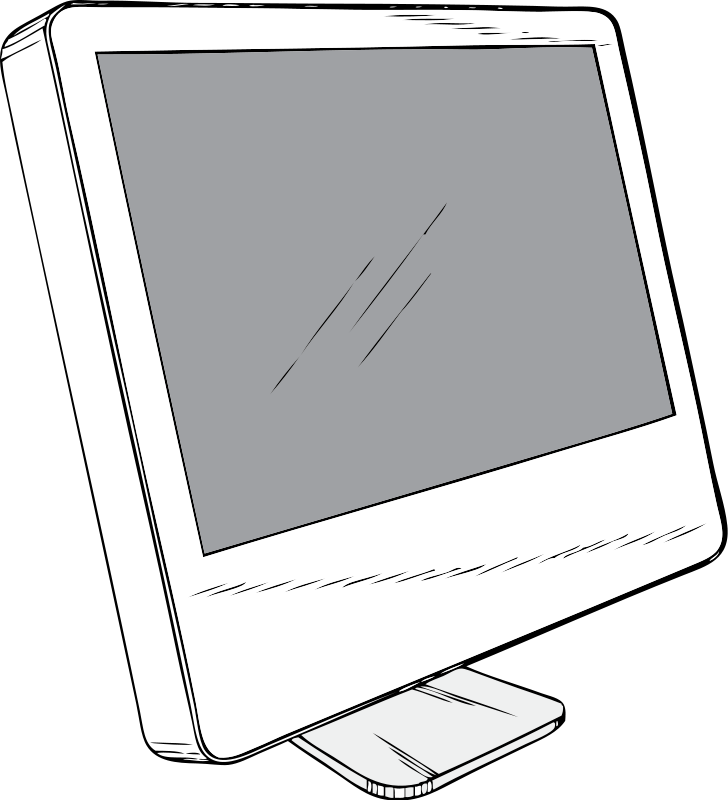
\includegraphics[height=1.5cm]{./monitor2.png}};   
    
    \node[fill=white, font=\scriptsize] at (virt.south) {Граница ВМ};
    
    \node[fill=white, font=\scriptsize] at (real.south) {Граница реальной системы};
\end{tikzpicture}

\end{frame}

\section{Постоянные хранилища}

\begin{frame}{Образы дисков}

Жёсткие диски
\begin{itemize}
\item RAW
\item VMDK, VDI, Qcow2, CRAFF, HDD, VHD\dots
\end{itemize}

\centering

\vfill

\begin{tikzpicture}[>=latex, font=\small, scale=0.5]
    \path (0,0.5) coordinate (a1);
    \draw (0,0) rectangle (7.5,1);
    \node[left = 0.25cm of a1] (host-disk) {Хозяйский диск};
    
    \draw (3,-2) rectangle (7,-1);
    \node[below = 0.7cm of host-disk] {Гостевой диск};
    
    % \draw[fill=black!5] (3,0) rectangle (6,1);
    % \draw[dotted] (3,-1) -- (3,0);
    % \draw[dotted] (6,-1) -- (6,0);
    
    \path[thick, fill=black!25] (1.2,0) rectangle (1.49,1);
    \path[fill=black!20] (1.51,0) rectangle (2.49,1);
    \path[fill=black!20] (2.51,0) rectangle (3.5,1);
    
    \path[fill=black!20] (4.,-2) rectangle (4.99,-1);
    \path[fill=black!20] (5.01,-2) rectangle (6,-1);
    
    \draw[<->] (4.25,-1) -- (2,0);
    \draw[<->] (5.25,-1) -- (3,0);
    
    \path (4.5,-2) coordinate (a2);
    \node[below =0.25cm of a2, inner sep=1pt] (used) {Используемые области};
    
    \draw[dotted] (used) -- (4.25,-2);
    \draw[dotted] (used) -- (5.25,-2);
    
    \draw[decorate, decoration={brace, amplitude=3pt}, yshift=3pt] (1.2,1) -- (3.5,1) coordinate[midway] (a3);
    \path (1.35,1) coordinate (a4);
    \node[above = 0.1cm of a3] {Образ диска};    
    \node[above = 0.5cm of a4, xshift=-2cm, inner sep=1pt] (header) {Заголовок};    
    \draw[dotted] (a4) -- (header);
    
\end{tikzpicture}

\end{frame}

\begin{frame}{Образы дисков}

Оптические диски CD/DVD/Blueray
\begin{itemize}
\item RAW для ISO 9660
\item Существует множество форматов, но они не используются в симуляторах или ВМ:
NRG, MDF, ISZ, DMG, IMG\dots
\end{itemize}

Гибкие диски
\begin{itemize}
\item 360 кБ — 2,88 МБ; Формат — RAW
\end{itemize}

\end{frame}

% \begin{frame}[allowframebreaks]{Последовательный порт}

% \begin{itemize}
% \item Простое устройство
% \item Модель добавляется одной из первых
% \item Поддерживается всеми ОС
% \item Малая скорость (до 115 кбит/с)
% \item Имеет современные реинкарнации (HSUART, SOL)
% \end{itemize}

% Со стороны реальной системы может быть присоединён к
% \begin{itemize}
% \item Реальному COM порту
% \item Виртуальному COM порту
% \item Именованному каналу (pipe)
% \item Сетевому сокету
% \item Эмуляторы терминала
% \item Файлу
% \end{itemize}

% \end{frame}

\section{Волшебная инструкция}

\begin{frame}[allowframebreaks]{Волшебные инструкции}

\begin{itemize}
\item Инструкция процессора с побочными эффектами
\item Остановка симуляции
\item Вызов обработчика, имеющего доступ к состоянию симулируемой системы
\item Изменение состояния
\item Возобновление симуляции
\item Для VM действия происходят «мгновенно»
\end{itemize}

Очень желательно, чтобы инструкция не встречалась в «обычном» коде

\begin{itemize}
\item Непривилегированная
\item Идеально, чтобы она вообще не имела эффектов вне симуляции
\item NOP — хороший кандидат
\item … но она используется в программах очень часто (ложные срабатывания)
\end{itemize}

Варианты
\begin{itemize}
\item NOP с префиксами/аргументами
\item В IA-32 есть «длинный NOP», от 1 до 9 байт
\item CPUID — в Simics для IA-32 (т.к. вызывает VM-exit)
\item Недокументированные инструкции (если ещё остались)
\end{itemize}

Использование:
\begin{itemize}
\item Инструментация приложений
\item Передача данных (по одному слову)
\item Канал управления для механизма RPC
\end{itemize}

\end{frame}

\begin{frame}{Не очень волшебные инструкции}

Специальные привилегированные инструкции для явного взаимодействия гостя-хозяина 
или минимизации накладных расходов для частых операций

\begin{itemize}
\item Hypercall, по аналогии с SYSCALL. В IA-32 - VMCALL
\item Кооперация по управлению виртуальной памятью. В IA-32: \#VE и VMFUNC
%\item
\end{itemize}

\end{frame}

\begin{frame}{Паравиртуальные устройства}

\begin{itemize}
\item Объём передаваемых данных за один раз больше
\item Ненастоящее устройство в карте памяти модели
\item Требует модификации гостевой ОС: драйвера устройств
\item Типичные кандидаты — устройства с большой пропускной способностью: диски,
сетевые карты
\item Пример: VirtIO~\cite{virtio}
\end{itemize}

\end{frame}

\begin{frame}{Паравиртуальные сервисы}

Взаимодействие с сервисами гостевой ОС:
\begin{itemize}
\item Управление питанием и жизненным циклом ОС
\item Файловая система
\item Потребление физической памяти 
\item Консольный доступ
\item Синхронизация времени~\cite{virt-time}
\end{itemize}

Примеры: 
\begin{itemize}
\item Wind River Simics Agent/Matic, Simics hostfs
\item Oracle Virtualbox Guest Additions
\item VMWare ESX Tools
\item Microsoft Hyper-V Integration Services~\cite{hyper-v-is}
\end{itemize}

\end{frame}

\section{Проброс устройств}

\begin{frame}[allowframebreaks]{Проброс устройств (passthrough)}

Передача хозяйского устройства в эксклюзивное использование гостя

\begin{itemize}
\item Графическая карта
\item Сетевые карты
\item Прочие устройства (PCIe/USB)
\end{itemize}

Проблемы: устройство или хозяйская ОС могут быть против!

\begin{itemize}
\item Доступы в регистры устройства
\item Доступы устройства в память (DMA)
\item Доставка прерываний от устройства
\end{itemize}


Дополнительные проблемы:

\begin{itemize}
\item Отключение устройства от хозяина
\item Графика и прочие legacy-особенности
\item Сохранение-восстановление и миграция состояния
\end{itemize}


\begin{itemize}
\item Аппаратная поддержка (I/O Memory management unit)
\item Intel VT-d, AMD IOMMU, IBM Translation Control Entry, Sun DVMA
\end{itemize}

\end{frame}

\section{Сеть}

\begin{frame}{Сетевое взаимодействие}

\begin{itemize}
\item Изначально создано для связи систем различной природы
\item Агностично к аппаратуре
\item Можно выбирать уровень абстракции, на котором будет проходить граница миров
\end{itemize}

Недостаток: требуется рабочий сетевой стек в госте
\end{frame}

\begin{frame}{Передача данных на разных уровнях модели OSI/ISO}

{\small
\begin{itemize}
\item Прикладной уровень — сервис-точки внутри симуляции. Отвечают на запросы гостя по конкретному прикладному протоколу: NFS, FTP, Samba, DHCP… 
\item Представительный уровень
\item Сеансовый уровень 
\item Транспортный уровень — NAT. Пакеты ретранслируются от имени хозяина. Входящие пакеты по умолчанию не доходят
\item Сетевой уровень — TUN-драйвер хозяина. Создаёт IP туннель
\item Канальный уровень — TAP-драйвер хозяина. Создаёт псевдоустройство Ethernet хозяина  
\item Физический уровень — модель карты внутри симуляции
\end{itemize}
}

\end{frame}

\section{Демо}

\begin{frame}{Демо на VirtualBox}


\end{frame}

\begin{frame}{Что осталось за рамками лекции}

\begin{itemize}
\item Chroot
\item Containers
\item PAL/SAL уровень
\item paravirt_ops \cite{lwn1, lwn2} 
\end{itemize}

\end{frame}

\begin{frame}{На следущей лекции}

Контрольная работа

% Языки моделирования и описания аппаратуры

\end{frame}


\section{Литература}

\begin{frame}[allowframebreaks]{Литература}
\begin{thebibliography}{99}
    \bibitem{tuntap}  \url{http://www.kernel.org/pub/linux/kernel/people/marcelo/linux-2.4/Documentation/networking/tuntap.txt}

    \bibitem{xen-passthrough} \url{http://wiki.xen.org/wiki/Xen_PCI_Passthrough}
        \url{http://wiki.xen.org/wiki/XenVGAPassthrough}
        \url{http://wiki.xen.org/wiki/XenUSBPassthrough}

    \bibitem{virt-time} Виртуальное время, часть 2: вопросы симуляции и виртуализации \url{http://habrahabr.ru/company/intel/blog/260119/}
    \bibitem{lwn1} \url{http://lwn.net/Articles/194339/}
    \bibitem{lwn2} \url{http://lwn.net/Articles/225881/}
    \bibitem{hyper-v-is} \url{https://technet.microsoft.com/en-us/library/dn798297.aspx}
    \bibitem{virtio} \url{http://www.linux-kvm.org/images/d/dd/KvmForum2007$kvm_pv_drv.pdf}
\end{thebibliography}
\end{frame}


\section{Конец}

\finalslide

\end{document}
